\section{Retrieving Images in Clusters}
\label{sec_introduction}

\todo{introduce the introduction?}

\subsection{Problem Statement \& Motivation}
training data for image categorization and content detection \\
flickr and other online photo communities are good sources for annotated images \\
problems: low annotation quality, only search for specific term (with different meanings and visual characteristics) \\
for example, want to test the quality of my algorithm in identifying different foods: would have to think of all kinds of food, then search images and group them into homogeneous groups manually

\bigskip

\emph{What do we do?} \\
clustering: creating homogeneous groups of semantically and visually similar pictures \\

\emph{Why do we do that?} \\
seminar challenge: cluster 1 million pictures of the MIR1M flickr file  \todo{what is flickr? folksonomy etc.} set \\
improving the complex task of searching for pictures according to a given keyword \\
facing different challenges like: multiple meanings of the keyword, bad picture annotations, taking semantic and visual information of a picture into account \\

\subsection{Clustered Tree Nodes Approach}
We implemented a web application in Python using SimpleCV\footnote{http://www.simplecv.org} for visual image analysis and Flask\footnote{http://flask.pocoo.org/} for the frontend.\\
The tool provides ready-to-use semantically and visually homogeneous image clusters for a given topic. This is achieved by first spanning a tree of subordinate terms, retrieving related images by their keywords for each term, and then clustering the images by their predominant keywords as well as by colors and edge structure. These two major phases are illustrated in figure \ref{fig_overallprocess}

\begin{figure}[h]
\centering
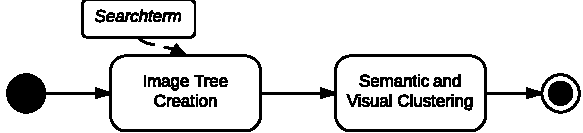
\includegraphics[]{images/search_process_highlevel.pdf}
\caption{The two main phases of our algorithm}
\label{fig_overallprocess}
\end{figure}

\bigskip

After giving an overview of Related Work in chapter 2, we will present how we analyze the image annotations and the user's search term to retrieve relevant images (chapter 3). Our methods to cluster these semantically and visually are described in chapter 4. Chapter 5 explains how we evaluate our approach, while the evaluation results will be discussed in chapter 6. At last, chapter 7 gives ideas for improvement and possible future work.
